\chapter{Simulação Distribuída}

Este trabalho enfoca os modelos estocásticos e de estados discretos, uma vez que eles são os que melhor representam modelos de sistemas computacionais.

Um sistemas de simulação sequencial, onde uma única máquina executa toda a simulação, pode ser retratado como uma fila de eventos aguardando para serem tratados. Cada evento possui o seu tempo de execução, como pode ser visto na figura~\ref{fig:simul}, que deve ser obedecido para garantir consistência do resultado.

Neste modelo sequencial, o sistema responsável pela simulação retira o próximo evento da fila de execução para tratá-lo. Ao fim do processamento, um próximo evento é retirado da fila, e isto se repete até o final de lista de eventos futuros. O tratamento de um evento pode ou não resultar dados que sejam necessários em um processamento futuro.

\begin{figure}
  %\centerline{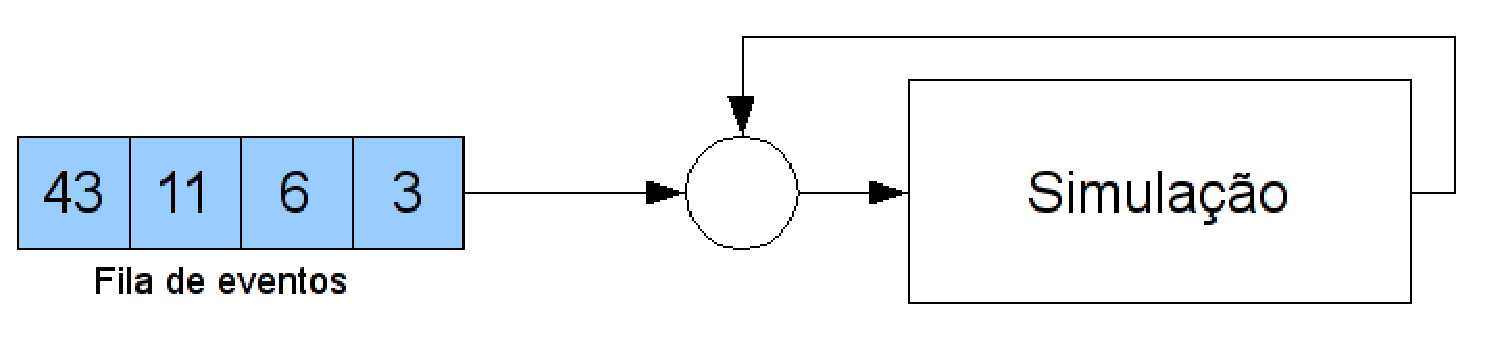
\includegraphics[scale=0.6]{simulacao.eps}}
  \caption{Simulação Sequencial.}
\label{fig:simul}
\end{figure}

\section{Simulação Distribuída}
A simulação é um processo que apresenta um custo computacional muito alto, tendo em vista a grande quantidade de dados que devem ser processados e a complexidade dos modelos matemáticos empregados. Esses fatores em conjunto podem encarecer computacionalmente o sistema, levando à ineficiência da simulação.

Uma das formas encontradas para se solucionar estes problemas foi dividir o tratamento dos diversos eventos entre vários processadores de uma mesma máquina paralela ou sobre um sistema distribuído, dando origem assim à Simulação Distribuída.

Distribuindo os eventos, reduz-se o tempo gasto pelos programas de simulação, mas, em contrapartida, novas situações necessitam de observação devido às características deste tipo de aplicação. É preciso sanar os problemas com a sincronização dos processos, sobrecarga da rede de comunicação, necessidade de balanceamento de carga do sistema, dentre outros.

Em um sistema de Simulação Distribuída, três estruturas devem ser observadas no desenvolvimento da simulação orientada à eventos:

\begin{itemize}
    \item As variáveis que descrevem os estados do sistema;
    \item Uma lista de eventos futuros, que contém os eventos a serem executados;
    \item Um relógio Global, que controla o progresso da simulação.
\end{itemize}

Os eventos devem ser executados obedecendo o seu \textit{timestamp}. O programa de simulação deve remover repetidamente da fila o evento com a menor marca de tempo e executá-lo. Assim que um evento é retirado da fila de execução, o relógio global avança para o tempo de ocorrência do evento. Esse mecanismo garante que todos os eventos sejam executados obedecendo a ordem cronológica do tempo de simulação. Porém, em se tratando de um sistema distribuído, não há como haver uma fila única de eventos. Portanto, o sistema passa a ser dividido em $n$ processos denominados $p_{1}, p_{2},\ldots, p_{n}$, cada um representando um processo do sistema real. Novos mecanismos devem ser incorporados ao sistema de simulação para garantir que cada evento seja executado na sua devida ordem.

Para cada processo lógico é atribuído um relógio que indica o seu progresso na simulação. A comunicação entre os processos se dá através mensagens, uma vez que não há áreas de memória compartilhadas entre os processos. Estas mensagens são também responsáveis pela sincronização do sistema. Caso algum evento $e_b$ venha a ocorrer antes de um segundo evento $e_a$, e sendo $a < b$, tem-se assim um erro de causa e efeito. Como em um sistema real nunca existirá tal situação, isto caracteriza uma inconsistência na simulação.

Os conceitos de sincronização de processos levaram ao desenvolvimento de protocolos, classificados como conservativos ou otimistas, para garantir a sincronização dos processos da simulação distribuída, evitando ou corrigindo erros de causa e efeito \cite{FUJIMOTO}.
